\section{Evaluation on Different Analysis Tasks}\label{sec:analysis-tasks}

\begin{table}[t]
	\caption{Data sets used in experiments. More data sets are included in the
	supplementary materials. In the main paper, every volume is of dimensions $64^3$. In the 
	supplementary materials, most volumes are of dimensions $256^3$.}
  \centering
  \begin{tabular}{p{0.08\textwidth}p{0.25\textwidth}p{0.12\textwidth}}
  \hline
  Name & Type & Data type \\
  \hline
  boiler & combustion simulation& float64\\
  plasma & magnetic reconnection simulation& float32\\
  diffusivity & hydrodynamics simulation& float64\\
  pressure & hydrodynamics simulation& float64\\
	turbulence & fluid dynamics simulation& float32\\
	kingsnake & CT scan & uint8\\
	foam & Scan? & uint16\\
	% flame & fluid dynamics simulation& float32 & x & x & x & x & x & Done\\
	% csafe & fluid dynamics simulation& uint8 & x &  &  & x & x & Done\\
	% enzo-v & fluid dynamics simulation& float32 & x & x &  & x &  & D(work2nd)\\
	% brain & fluid dynamics simulation& uint8 & x &  &  & x & x & Done\\
	% foam & fluid dynamics simulation& uint16 & x & x & x & x & x & Done\\
	% vismale & fluid dynamics simulation& uint8 & x & x & x & x & x & P(rerun)\\
	% karfs	& fluid dynamics simulation& float32 & x & x &  & x & x & Done\\
	% aneurism	& fluid dynamics simulation& uint8 & x & x &  & x & x & Done\\
  % velocityz & hydrodynamics simulation& float64 & x & x &  & x & x & D(main)\\
  \hline
  \end{tabular}\label{tbl:data-sets}
\end{table}

In this section, we consider a variety of common analysis tasks, namely function reconstruction
(\Cref{sec:rmse-optimized}), derivative computation (\Cref{sec:gradient,sec:laplacian}), histogram
computation (\Cref{sec:histogram}), and isocontour extraction (\Cref{sec:isocontour}). For each
task, we define an error metric $\err$ that is the basis for evaluating the performance of different
streams on the task. We use~\Cref{alg:greedy} to compute a stream $\sopt$ that is optimized for each
task, and use its signature to compute $\ssig$. We compare $\slvl$, $\sbit$, $\swav$, $\smag$,
$\ssig$, and $\sopt$ by evaluating the error as a function of the number of packets received. To
mimic the effects of entropy compression commonly used in practice, we remove all packets that
contain only leading zero bits from each stream before plotting. This comparison is performed on a
variety of data sets, listed in \Cref{tbl:data-sets}. The wavelet basis allows us to always
reconstruct data at full resolution, which greatly simplifies computations of errors (we are unaware
of standard methods to compute, for example, the root-mean-square error between grids of different
dimensions).

\subsection{Function Reconstruction}\label{sec:rmse-optimized}

\begin{figure*}[t]
\centering
 \subcaptionbox{\label{fig:rmse:boiler}\emph{boiler}}{{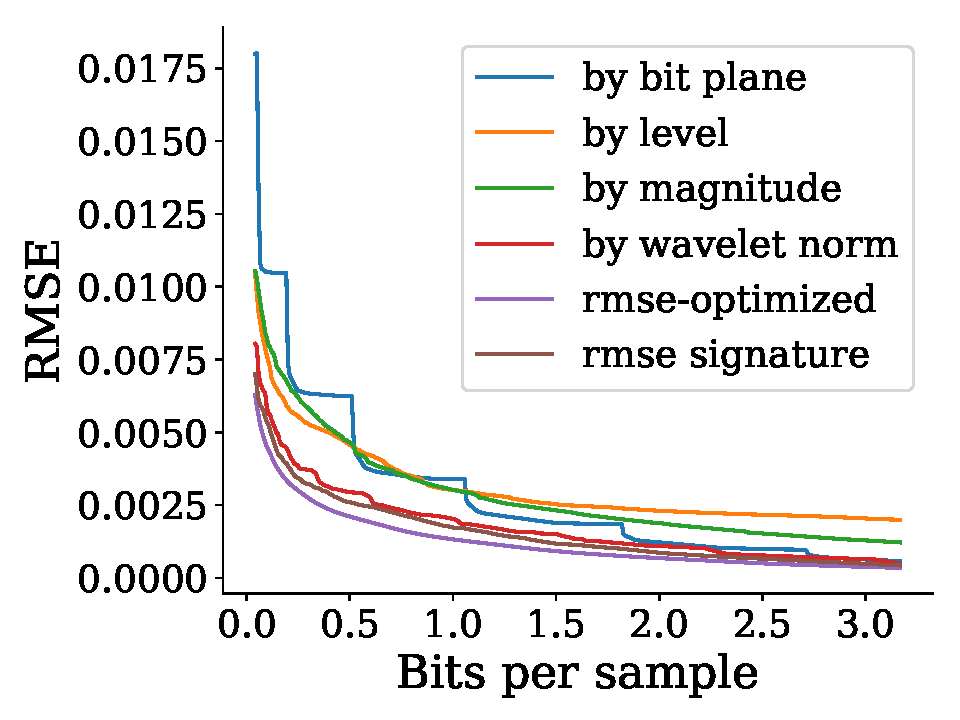
\includegraphics[width=0.24\linewidth]{rmse/rmse-optimized-boiler}}}
 \subcaptionbox{\label{fig:rmse:diffisivity}\emph{diffusivity}}{{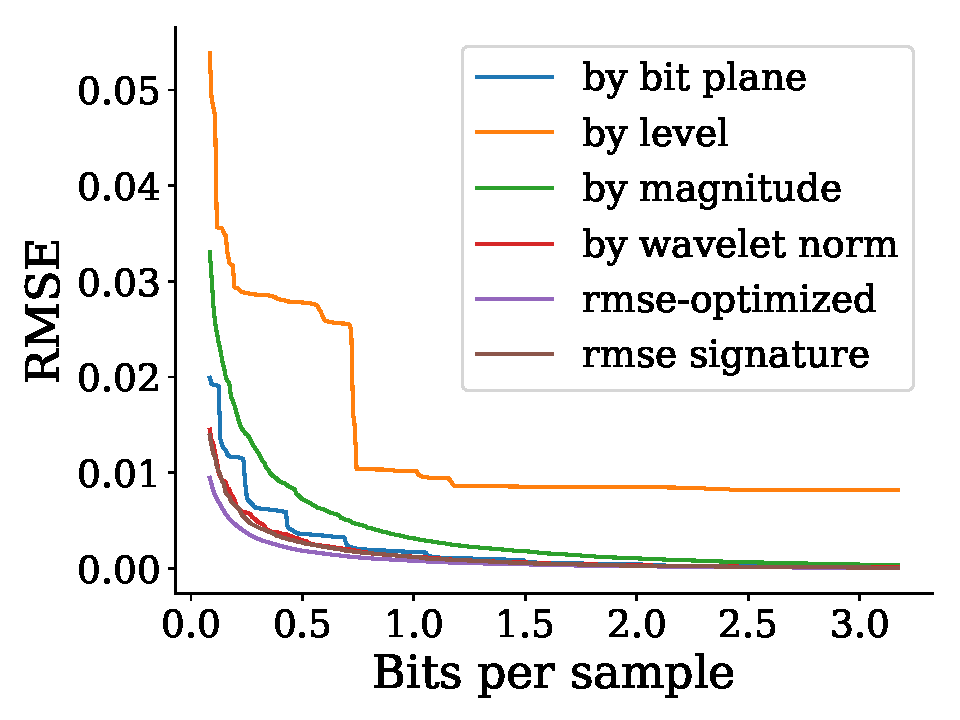
\includegraphics[width=0.24\linewidth]{rmse/rmse-optimized-diffusivity}}}
 \subcaptionbox{\label{fig:rmse:plasma}\emph{plasma}}{ {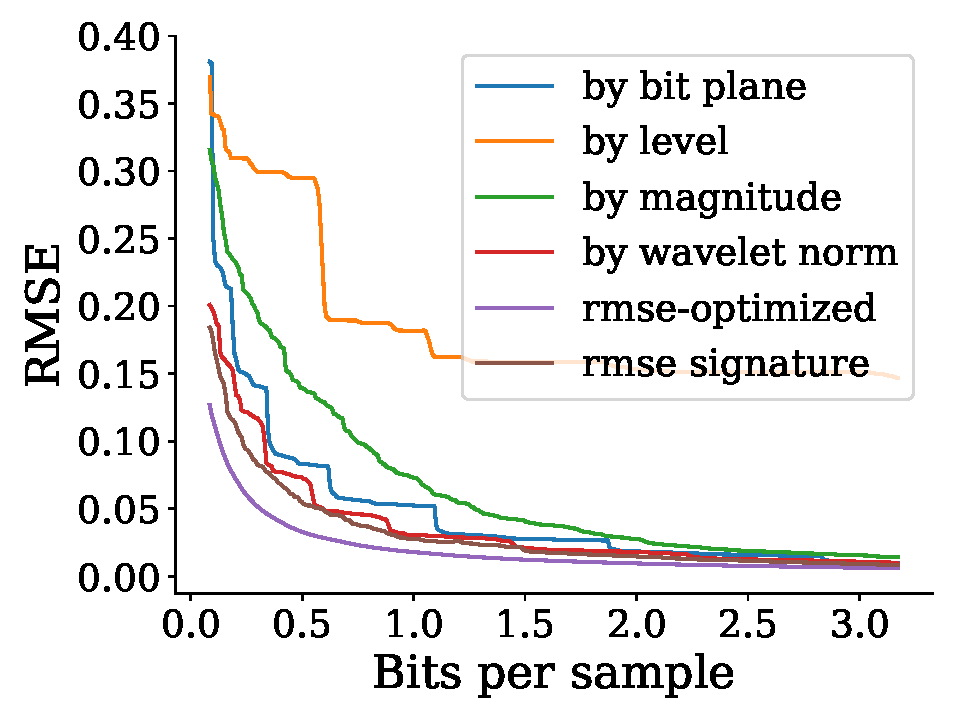
\includegraphics[width=0.24\linewidth]{rmse/rmse-optimized-plasma}}}
 \subcaptionbox{\label{fig:rmse:kingsnake}\emph{kingsnake}}{{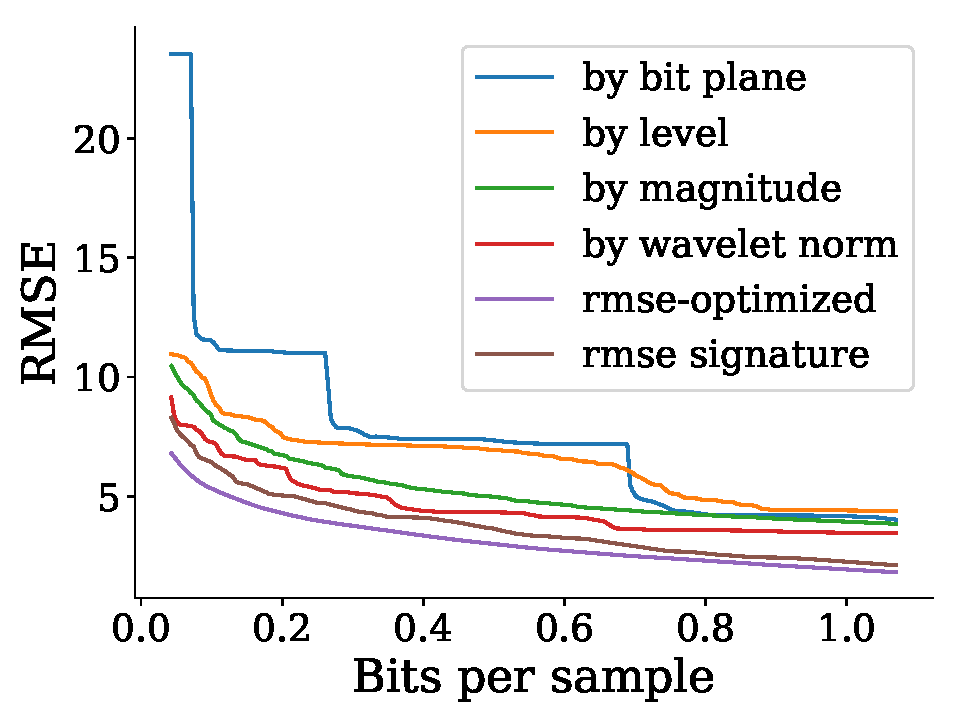
\includegraphics[width=0.24\linewidth]{rmse/rmse-optimized-kingsnake}}}
\caption{Root-mean-square error (RMSE) of reconstructed functions for different streams and data
sets; lower RMSE is better. The streams are truncated at both ends to highlight the differences,
without omitting important information. Leading zero packets are not used for plotting. The general
ordering of error, from lowest to highest, is $\sopt < \ssig < \swav < \sbit < \smag < \slvl$ (for
\emph{boiler} and \emph{kingsnake}, \sbit underperforms \slvl at first, but surpasses its after a
certain bit rate).}
\label{fig:rmse-optimized}
\vspace{1em}

\centering
 \subcaptionbox{\emph{by level} (\slvl)}{{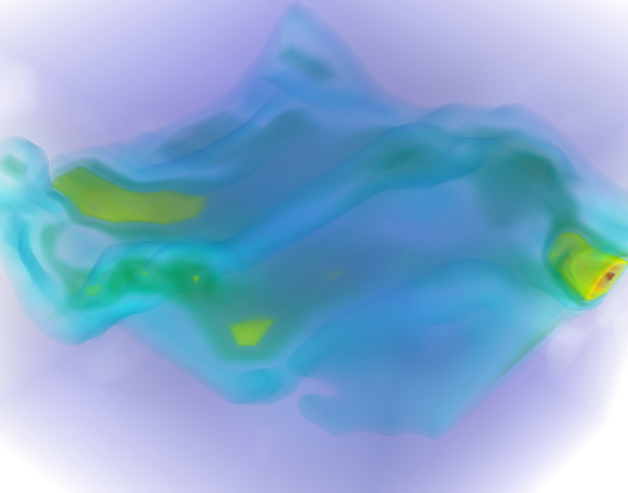
\includegraphics[width=0.16\linewidth]{rmse/rmse-plasma-level}}}
 \subcaptionbox{\emph{by bit plane (\sbit)}}{{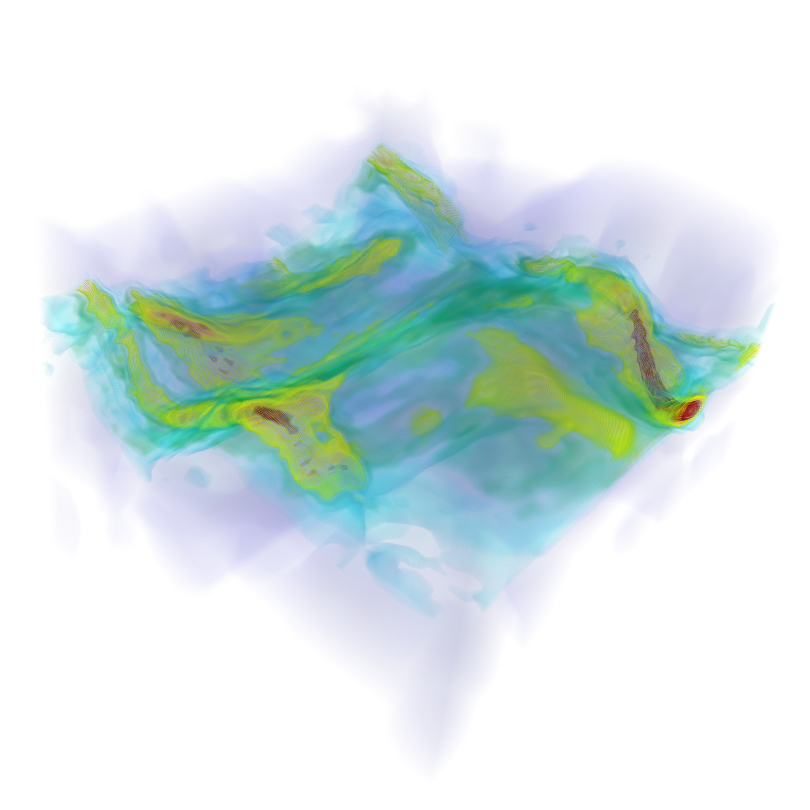
\includegraphics[width=0.16\linewidth]{rmse/rmse-plasma-bit-plane}}}
 \subcaptionbox{\emph{by wavelet norm (\swav)}}{{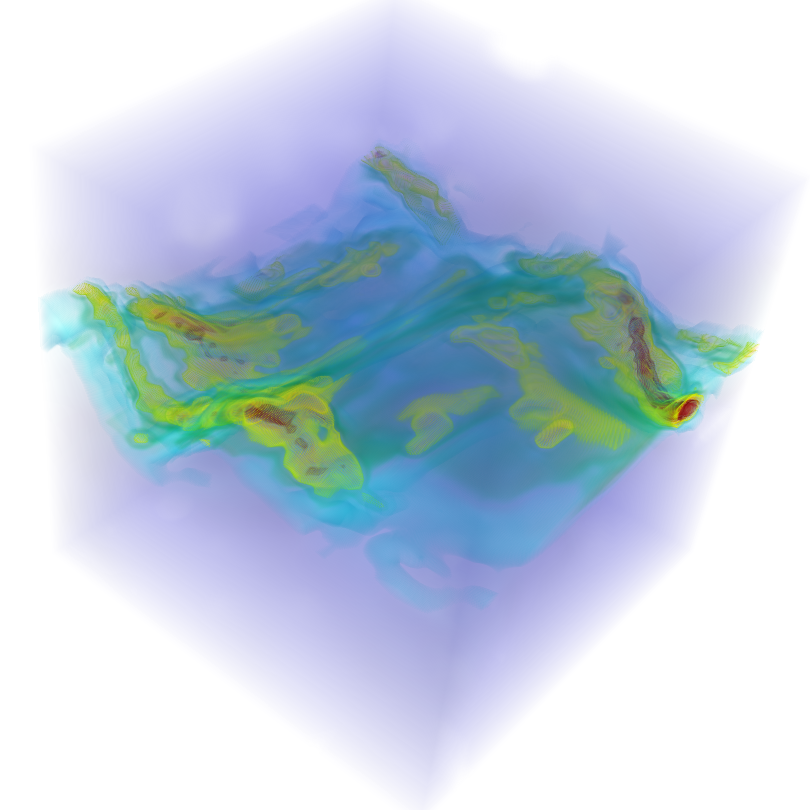
\includegraphics[width=0.16\linewidth]{rmse/rmse-plasma-wavelet-norm}}}
 \subcaptionbox{\emph{by magnitude (\smag)}}{{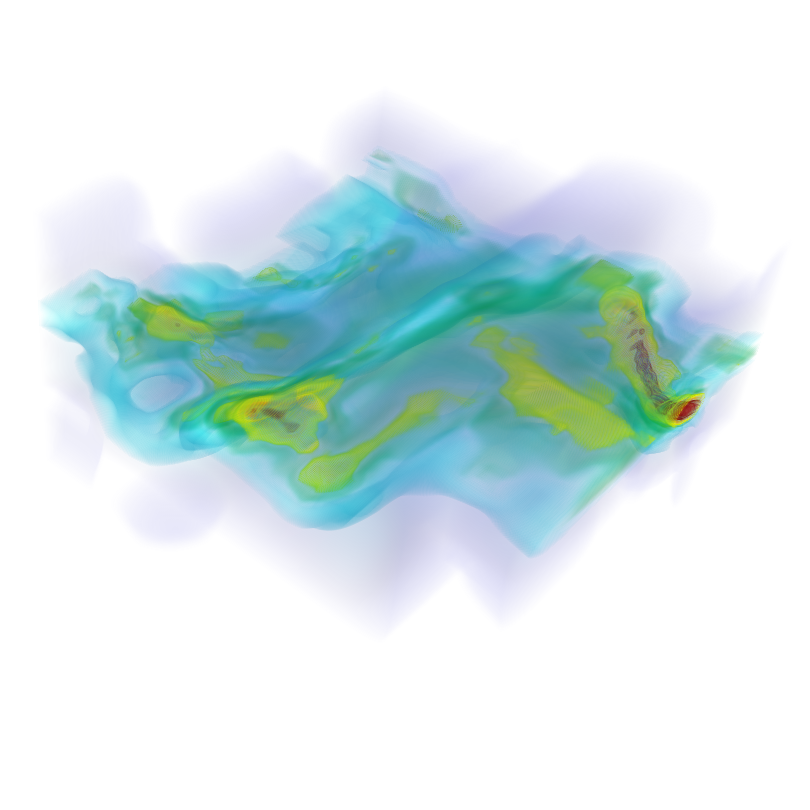
\includegraphics[width=0.16\linewidth]{rmse/rmse-plasma-magnitude}}}
 \subcaptionbox{\emph{by signature (\ssig)}}{{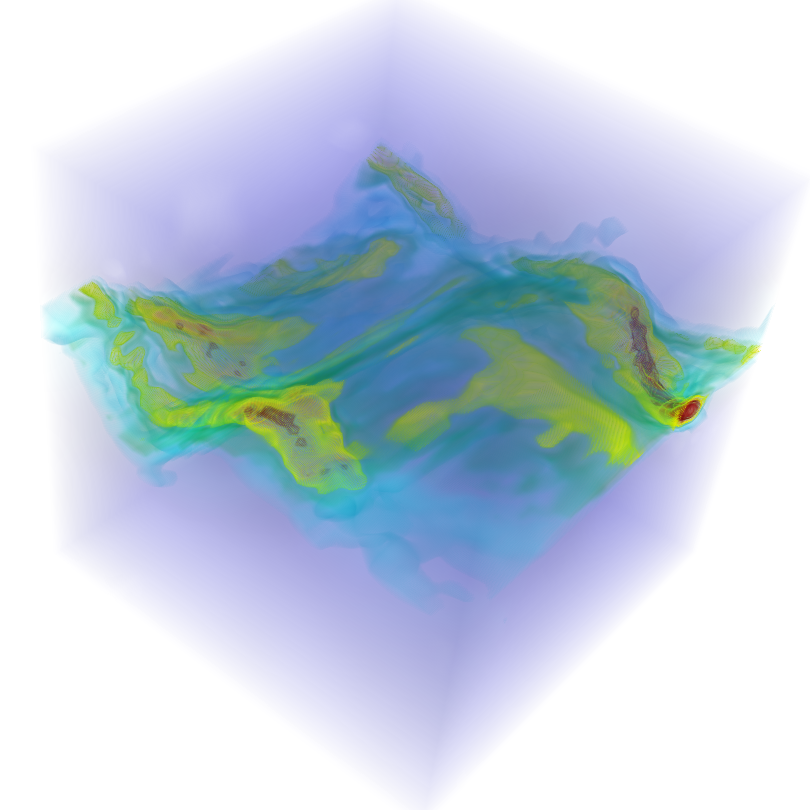
\includegraphics[width=0.16\linewidth]{rmse/rmse-plasma-signature}}}
 \subcaptionbox{\emph{ground truth}}{{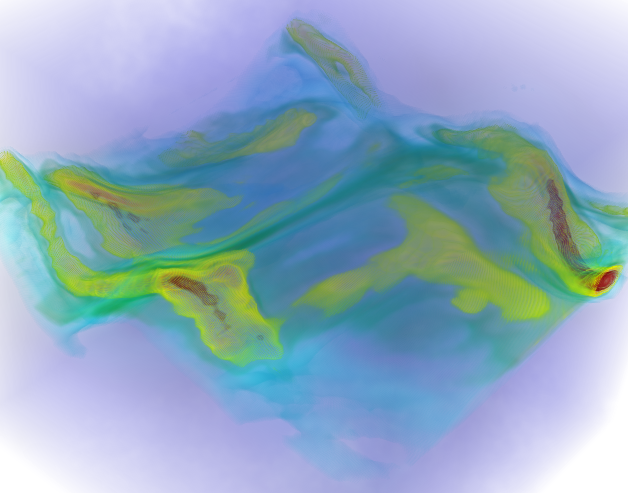
\includegraphics[width=0.16\linewidth]{rmse/rmse-plasma-groundtruth}}}
\caption{Volume renderings of a $64^3$ region of \emph{plasma} data set at 0.1 bps.  \slvl captures
the background (purple-blue) well, whereas \sbit captures the fine details better. \swav combines
the strength of both. \ssig, however, produces the most accurate rendering (compare, e.g., yellow
features).
\pavol{should we circle them or use an arrow?}\hb{yes, please}}
\label{fig:rmse-rendering}
\end{figure*}

One of the most fundamental analysis tasks is that of reconstructing the original function itself. A
commonly used error metric in this case is the root-mean-square error
(RMSE).~\Cref{fig:rmse-optimized} shows the comparison of the different streams for a variety of
datasets. It can be noted that, in general, $\sopt$ performs better than $\ssig$ due to spatial
adaptivity, whereas \ssig slightly outperforms \swav, followed by \sbit, \smag, and \slvl.

In particular, \sbit performs better than \slvl (for \emph{kingsnake} and \emph{boiler} it does so
after approximately 1 bps), which can be attributed to our removal of leading zero packets, because
empirically, wavelet coefficients on finer scale subbands are much smaller in magnitude(\todo{cite}).
Such coefficients contain a majority of the leading zero bits, whose removal benefits \sbit the
most, as it touches fine-resolution bits the earliest. Compared to \emph{kingsnake} and
\emph{boiler}, \emph{diffusivity} and \emph{plasma} contain a sigificant amount of empty space,
which translates to more leading zero bits after the wavelet transform, that \sbit can take
advantage of --- the number of leading zero packets are: 406,219 (\emph{kingsnake}), 380,955
(\emph{boiler}), 322,073 (\emph{plasma}), and 215,716 (\emph{diffusivity}). This is the reason why
unlike for \emph{boiler} and \emph{kingsnake}, \sbit outperforms \slvl immediately from the
beginning for \emph{diffusivity} and \emph{plasma}. 

\smag underperforms for the same reason that \slvl does, but to a lesser extent, since \smag is
better adaptive to the data. \swav outperforms both \slvl and \sbit, because it follows the optimal
(data-independent) bit ordering in $\strm_{L,B}$ in the $L_2$ norm, which is also the norm that RMSE
is based upon. Unsurprisingly, \sopt outperforms all the others, as it is the most data-adaptive
(i.e., it can prioritize packets in the spatial domain in addition to the $\strm_{L,B}$ domain).
\ssig is the second best stream, as it follows the bit ordering of \sopt in $\strm_{L,B}$, but lacks
any spatial adaptivity. In general, \swav and \ssig have similar performance. In some cases (e.g.,
~\Cref{fig:rmse:diffisivity} and~\Cref{fig:rmse:plasma}), \ssig is able to adapt more to the data,
thus outperforming \swav by a larger margin.

We explore the errors visually by volume rendering the \emph{plasma} data set at 0.1 bits per
sample, for all streams~(\Cref{fig:rmse-rendering}). Bits per sample (bps) are calculated by
dividing the total size of received packets (in bits) by the total number of samples. Although \slvl
has the precision to obtain an accurate background, it lacks resolution to resolve the fine details.
\sbit, instead, lacks the precision to reconstruct the (mostly smooth) background, but has enough
resolution to capture the fine details well. \swav balances both precision and resolution, producing
a more accurate picture as a whole. In this case, the \ssig stream manages to produce the most
accurate rendering. In general, \ssig benefits more from ``anisotropic'' data, such as
\emph{plasma}, where most features lie on a thin ``surface''. For such data, wavelet coefficients
along one dimension are often larger compared to those along other dimensions, which \sopt, and
hence \ssig, can take advantage of, but not \swav.
